% !TEX root = ../main.tex
\subsection{CLAS} \label{ssec::clas}
    \begin{figure}[htbp]
        \centering
        \fbox{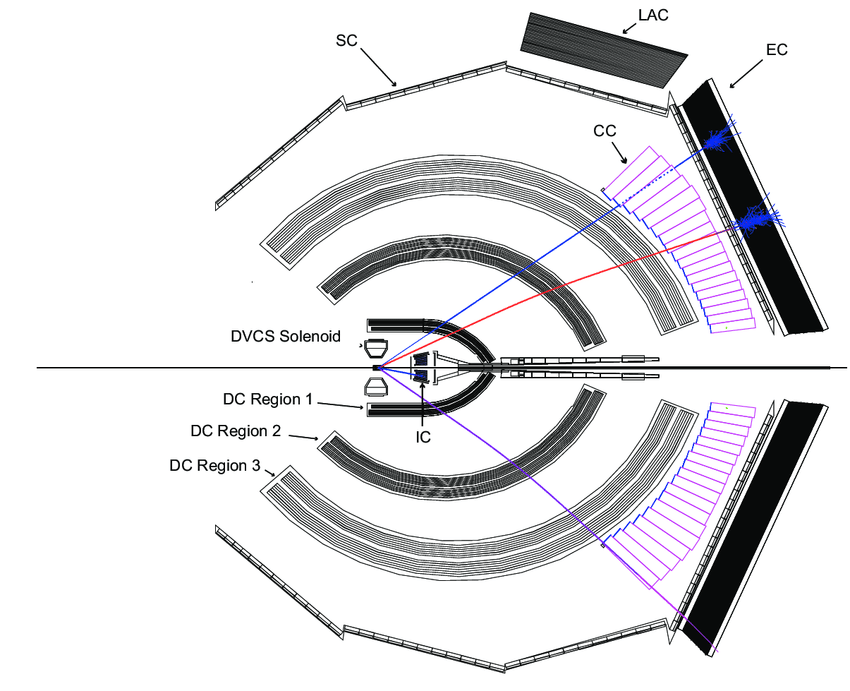
\includegraphics[width=0.8\textwidth]{11experiment/img/20clas.png}}
        \caption{\label{fig::clas} Schematic of CLAS. \\
        Source: \cite{bedlinskiy2014pi0}.}
    \end{figure}

    Particularly, in Hall B, the detector utilised up to 2005 (\textbf{TODO: PENDING CITATION}) is the CEBAF Large Accelerator Spetrometer (CLAS), where each particle-target collision --- denominated event --- is captured for analysis.
    This is done in an order of up to several thousand events per second, and the recorded data is later transferred to a farm of computing processors
    for High Energy Physics (HEP) analysis to be done on it.

    The design of CLAS is based on a toroidal magnetic field.
    This provides a momentum resolution of $\delta p/p \leq 0.5\%$~\cite{mestayer2000dc}.
    The design also has full azimuthal angle coverage and polar angle coverage from 8$\deg$ to 142$\deg$ relative to the direction of the incoming beam~\cite{mecking2003cebaf}.
    Thanks to this large angle acceptance for charged particles, CLAS is well suited for experiments that require the detection of two or more particles.
    
    CLAS is divided into six identical sectors, where each is an independent spectrometer.
    5-meter long superconducting coils of toroidal magnets separate each sector.
    These magnets produce a toroidal magnetic field which bends particles in only the polar direction.
    
    In CLAS experiments, it is standard for the field to force the particles to be in-bending compared to the direction of the beam.
    This is the case for the experiment that forms the basis of this work, EG2.
    
    A diagram of CLAS can be seen in figure \ref{fig::clas}.
    The inbending trajectories of the charged particles (in red and purple) can be seen.

    The particle detection system consists of five detectors which are designed to measure different properties of the particles from the reaction.
    These are Drift Chambers (DC), Cherekov Counters (CC), Time-Of-Flight (TOF), Scintillation Counters (SC), and Electromagnetic Calorimeters (EC).
    Each of these will be detailed in the following subsections.
    
    \input{11experiment/21dc}
    \input{11experiment/22cc}
    \input{11experiment/23sc}
    \input{11experiment/24ec}
